%%%%%%%%%%%%%%%%%%%%% Chapter 9 %%%%%%%%%%%%%%%%%%%%%%%%%%%%%%%%%
% Hardware-Rooted Trust: TEEs and Enclaves
%%%%%%%%%%%%%%%%%%%%%%%%%%%%%%%%%%%%%%%%%%%%%%%%%%%%%%%%%%%%%%%%%
\motto{TEEs provide confidential computing: data is encrypted not just at rest and in transit, but also during processing.}

\chapter{Hardware-Rooted Trust: TEEs and Enclaves}
\label{chap:tees_enclaves}

\abstract{In this chapter, we explore how to anchor trust in the physical hardware layer through Trusted Execution Environments (TEEs). While cryptographic methods like Homomorphic Encryption offer mathematical protection, they often carry prohibitive performance costs. TEEs, such as Intel SGX \cite{costan2016} and ARM TrustZone, provide a high-performance alternative by isolating sensitive AI workloads in secure enclaves. We analyze the core properties of TEEs---Confidentiality, Integrity, Attestation, and Isolation---and demonstrate how they can be combined with statistical and cryptographic defenses to create a robust, defense-in-depth architecture.}

\section{When Cryptography Is Not Enough}
\label{sec:crypto_limitations}

As we saw in the previous chapters, cryptographic defenses like Secure Aggregation and Homomorphic Encryption are powerful, but they come with significant limitations. The performance overhead of HE can be 100--1000x slower than plaintext computation, and key management remains a major operational challenge. Furthermore, cryptographic protocols often assume an "honest-but-curious" adversary, offering less protection against a malicious operating system or hypervisor.

Trusted Execution Environments (TEEs) solve these problems by shifting the root of trust from software to hardware. By isolating computation in secure enclaves, we can protect data "in use," ensuring that even if the host machine's OS is compromised, the sensitive AI model and user data remain inaccessible.

\section{Core Properties of a TEE}
\label{sec:tee_properties}

A TEE provides four fundamental security guarantees that are vital for a Trustworthy AI Architect:

\begin{description}
  \item[Confidentiality:] 
        Data inside the enclave is encrypted at the hardware level; it is inaccessible to the OS, hypervisor, or co-located processes.
  \item[Integrity:]
        The code inside the enclave is measured before execution and cannot be tampered with, ensuring the AI model has not been modified.
  \item[Attestation:]
        A remote party can verify the authenticity and state of the enclave before sending sensitive data to it.
  \item[Isolation:]
        Enclave memory is physically isolated from the rest of the system's memory, preventing side-channel leakage.
\end{description}

\begin{figure}[t]
\centering
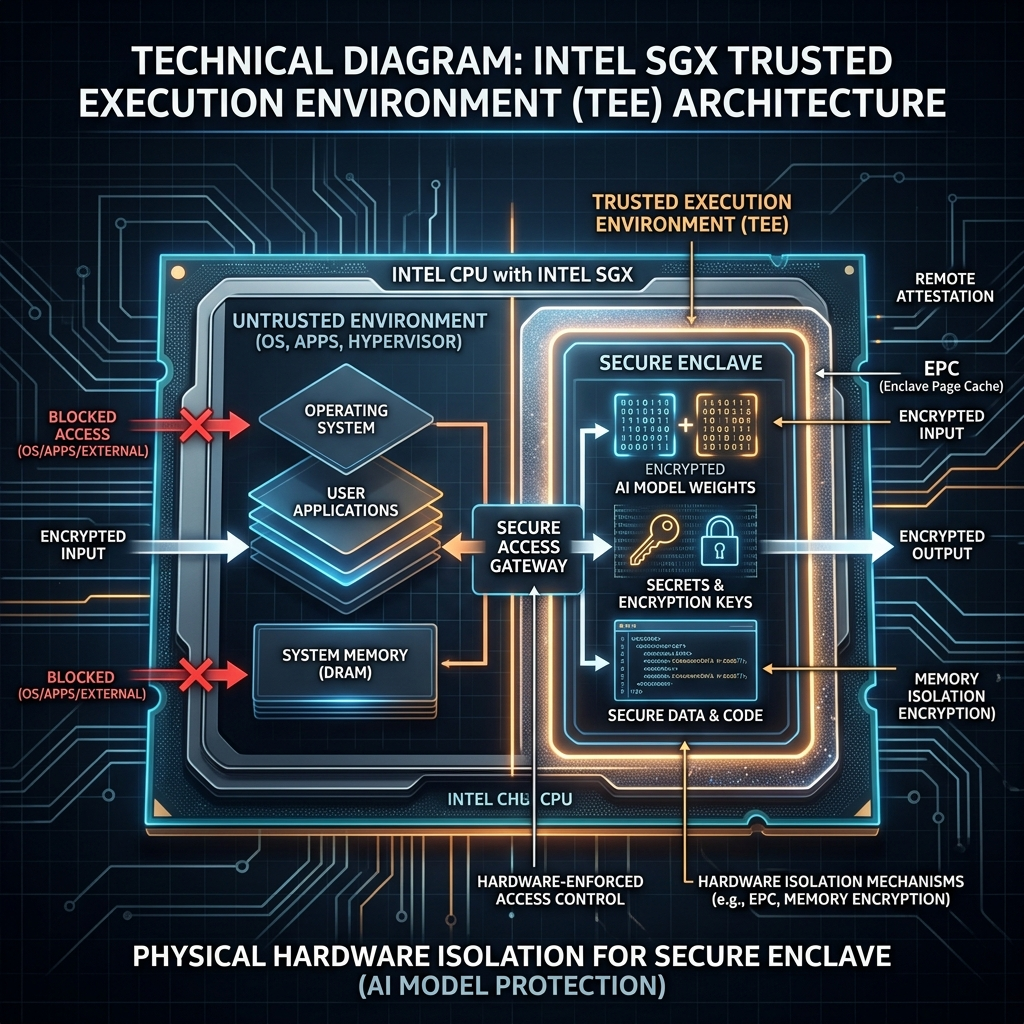
\includegraphics[width=\textwidth]{figures/ch9_tee.png}
\caption{Hardware-Rooted Trust: Architecture of a Trusted Execution Environment (TEE) showing the isolated Secure Enclave protecting data while in use.}
\label{fig:ch9_tee}
\end{figure}

\section{Major TEE Technologies}
\label{sec:tee_technologies}

Three primary technologies dominate the confidential computing landscape:

\begin{table}
\caption{Comparative Overview of TEE Technologies}
\label{tab:tee_tech}
\begin{tabular}{p{3cm}p{1.5cm}p{6cm}}
\hline\noalign{\smallskip}
Technology & Vendor & Best For \\
\noalign{\smallskip}\svhline\noalign{\smallskip}
Intel SGX & Intel & Server-side confidential AI and model serving. \\
ARM TrustZone & ARM & Mobile and IoT edge AI; on-device inference. \\
AMD SEV & AMD & Virtual machine-level isolation in the cloud. \\
\noalign{\smallskip}\hline\noalign{\smallskip}
\end{tabular}
\end{table}

In emerging markets like ASEAN, \textbf{ARM TrustZone} is particularly critical due to its ubiquity in the smartphones and IoT devices that power local digital economies.

\section{Defense-in-Depth: The Composition of Trust}
\label{sec:tee_composition}

A truly resilient architecture does not rely on a single layer. The most secure systems utilize a composition of defenses:
\begin{equation}
\text{Total Protection} = \underbrace{\text{TEE}}_{\text{Hardware}} + \underbrace{\text{DP } (\epsilon, \delta)}_{\text{Statistical}} + \underbrace{\text{SecAgg}}_{\text{Cryptographic}}
\end{equation}

In this stack, the TEE protects the computation, Secure Aggregation protects the transit, and Differential Privacy protects the final output from being reverse-engineered.

\section{Practical Implementation: Secure Inference}
\label{sec:tee_implementation}

To implement secure inference inside an enclave (e.g., using the Open Enclave SDK), the architect must ensure that sensitive data only exists in plaintext within the enclave's "trusted" memory. Before leaving the enclave, all outputs must be re-encrypted, and the internal memory must be explicitly cleared to prevent any residual traces.

\section{Conclusion}
\label{sec:conclusion_tees}

By rooting trust in hardware, we enable AI to process sensitive data in environments we do not fully trust---such as public clouds or potentially compromised edge devices. However, hardware trust assumes a cooperative infrastructure. In the next chapter, we address the possibility of adversarial infrastructure through \textbf{Robust Aggregation}, ensuring the global model survives even when participants are actively malicious.


